\chapter{Intégration SIEM avec Wazuh}

\section{Présentation de Wazuh}

Wazuh est une plateforme SIEM open-source (fork d'OSSEC) offrant une analyse en temps réel des événements de sécurité, une détection d'intrusion basée sur des règles et une conformité réglementaire (PCI-DSS, GDPR)~\cite{wazuh_docs}. Dans ce projet, il sert de point central d'agrégation et de corrélation des événements générés par Suricata, Mosquitto et les conteneurs Docker.

Le diagramme de composants de la figure~\ref{fig:wazuh_pipeline} illustre le pipeline d'ingestion et de traitement des événements dans Wazuh.

\begin{figure}[H]
  \centering
  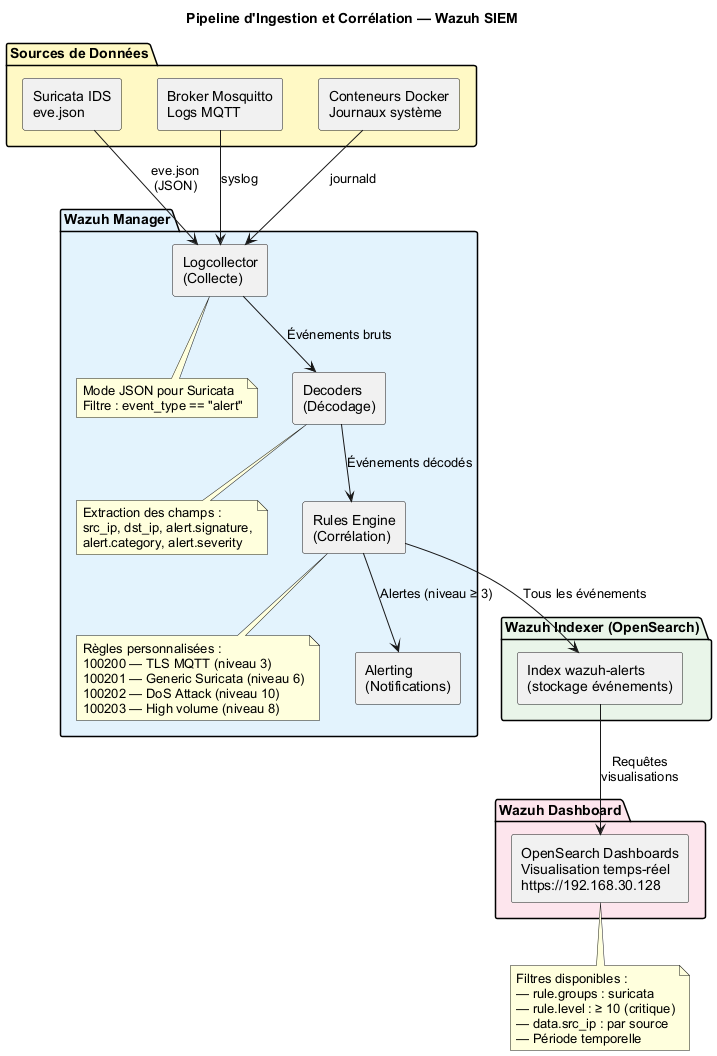
\includegraphics[width=\textwidth]{diagrams/diag-wazuh-pipeline.png}
  \caption{Pipeline d'ingestion et de traitement Wazuh}
  \label{fig:wazuh_pipeline}
\end{figure}

\section{Déploiement de Wazuh OVA}

\subsection{Choix du mode de déploiement}

Après avoir évalué l'option Docker Compose (qui présentait des incompatibilités avec l'environnement GNS3), le déploiement final retenu est l'OVA officielle Wazuh v4.7 sur VMware Workstation Pro.

\begin{table}[H]
\centering
\caption{Configuration de la VM Wazuh}
\label{tab:wazuh_config}
\begin{tabular}{ll}
\toprule
\textbf{Paramètre} & \textbf{Valeur} \\
\midrule
Adresse IP & 192.168.30.128 \\
RAM & 8~Go \\
vCPU & 4 \\
Stockage & 50~Go \\
Dashboard & \texttt{https://192.168.30.128} \\
\bottomrule
\end{tabular}
\end{table}

\subsection{Architecture Wazuh}

La solution Wazuh déployée comprend une architecture \textit{single-node} :
\begin{itemize}
  \item \textbf{Wazuh Manager} : Moteur de règles, corrélation, agrégation.
  \item \textbf{Wazuh Indexer} : Stockage et indexation (OpenSearch).
  \item \textbf{Wazuh Dashboard} : Interface de visualisation (OpenSearch Dashboards).
\end{itemize}

\section{Configuration de l'ingestion Suricata}

\subsection{Logcollector}

Le Wazuh Manager est configuré pour surveiller le fichier EVE JSON de Suricata en mode \texttt{tail}. Seuls les événements de type \texttt{alert} sont ingérés, via un filtre JSON sur le champ \texttt{event\_type}. La configuration du module \texttt{localfile} est détaillée en Annexe~B.

\subsection{Règles de corrélation personnalisées}

Quatre règles personnalisées (IDs 100200-100203) ont été créées pour élever le niveau de sévérité des alertes Suricata et permettre la corrélation multi-sources :

\begin{table}[H]
\centering
\caption{Règles Wazuh personnalisées pour les alertes IoT}
\label{tab:wazuh_rules}
\begin{tabular}{clcl}
\toprule
\textbf{Rule ID} & \textbf{Description} & \textbf{Niveau} & \textbf{Déclencheur} \\
\midrule
100200 & TLS MQTT traffic & 3 (Low) & Trafic Suricata sur port 8883 \\
100201 & Generic Suricata alert & 6 (Medium) & Alerte Suricata sévérité 1-3 \\
100202 & DoS Attack detected & 10 (Critical) & Catégorie ``Denial of Service'' \\
100203 & High volume alerts & 8 (High) & 10+ alertes par source en 60~s \\
\bottomrule
\end{tabular}
\end{table}

La règle 100203 utilise le mécanisme de \textbf{corrélation} de Wazuh : elle se déclenche lorsque 10~alertes ou plus proviennent de la même adresse IP source dans un intervalle de 60~secondes, signalant une activité malveillante soutenue. Le texte complet des règles XML est fourni en Annexe~B.

\section{Visualisation dans le dashboard}

\subsection{Dashboard Wazuh -- résultats}

Les 51 alertes Suricata ont été correctement ingérées et indexées dans Wazuh. Elles sont visibles via le filtre \texttt{rule.groups: suricata} dans l'interface de découverte.

\begin{figure}[H]
  \centering
  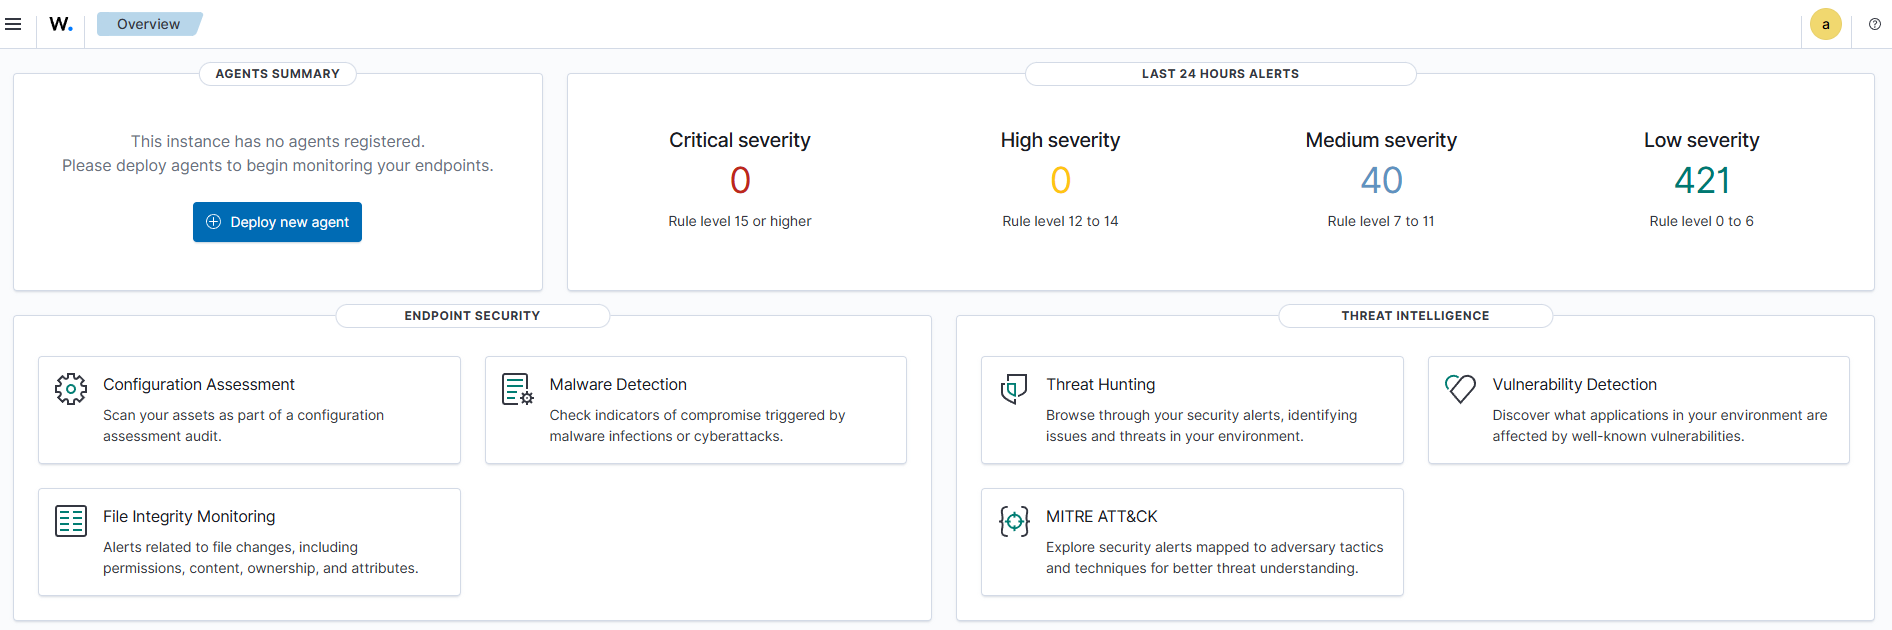
\includegraphics[width=\textwidth]{figures/wazuh-dashboard.png}
  \caption{Dashboard Wazuh affichant les alertes IoT/MQTT}
  \label{fig:wazuh_dashboard}
\end{figure}

\subsection{Distribution des alertes par niveau}

\begin{table}[H]
\centering
\caption{Distribution des alertes par niveau de sévérité Wazuh}
\label{tab:wazuh_levels}
\begin{tabular}{lll}
\toprule
\textbf{Niveau} & \textbf{Règle} & \textbf{Alertes} \\
\midrule
3 (Low) & 100200 -- TLS MQTT & 18 \\
6 (Medium) & 100201 -- Generic Suricata & 20 \\
8 (High) & 100203 -- High volume & 9 \\
10 (Critical) & 100202 -- DoS Attack & 4 \\
\bottomrule
\end{tabular}
\end{table}

\begin{resultbox}[Résultats Wazuh SIEM]
\begin{itemize}
  \item \textbf{51 alertes Suricata} ingérées et indexées avec succès.
  \item \textbf{4 alertes critiques} (niveau 10) pour les attaques DoS -- escalade correctement appliquée.
  \item Corrélation multi-sources opérationnelle (Suricata + logs système).
  \item Dashboard visible à \texttt{https://192.168.30.128} avec visualisations temps-réel.
\end{itemize}
\end{resultbox}
